\documentclass[
	11pt, % Tamanho padrão da fonte
	% t, % Alinhar verticalmente ao topo
	% aspectratio=169, % Definir proporção 16:9    
]{beamer}

\usepackage[style=authoryear, backend=biber]{biblatex} % URL zu lang für Präsi
\addbibresource{SynthetischeDaten.bib}

% Caminho para imagens
\graphicspath{{img/}}

% Pacotes adicionais
%\usepackage[alf]{abntex2cite} % Citações ABNT
\usepackage{booktabs} % Linhas de tabela aprimoradas
\usepackage{palatino} % Fonte Palatino
\usepackage[default]{opensans} % Fonte Open Sans
\usepackage{hyperref}
\usepackage{xurl} % url in Quelle sonst zu groß
\usepackage{caption}
\usepackage[ngerman]{babel}


%----------------------------------------------------------------------------------------
%	SELEÇÃO DE LAYOUT E CORES
%----------------------------------------------------------------------------------------

\usetheme{Boadilla} % Tema de layout

% Definição de cores personalizadas
\definecolor{primaryColor}{RGB}{20,45,105} % Cor primária
\definecolor{secondaryColor}{RGB}{0,100,160} % Cor secundária

% Aplicação das cores no tema
\setbeamercolor{structure}{fg=primaryColor}
\setbeamercolor{palette primary}{bg=primaryColor, fg=white}
\setbeamercolor{palette secondary}{bg=secondaryColor, fg=white}
\setbeamercolor{title}{bg=primaryColor, fg=white} % Cor do título principal

% Cores no cabeçalho
\setbeamercolor{headline}{bg=secondaryColor, fg=white}
\setbeamercolor{section in head/foot}{bg=primaryColor, fg=white}
\setbeamercolor{subsection in head/foot}{bg=secondaryColor, fg=white}

% Configurações de cores para o rodapé
\setbeamercolor{author in head/foot}{bg=primaryColor, fg=white} % Nome
\setbeamercolor{title in head/foot}{bg=secondaryColor, fg=white} % Título
\setbeamercolor{date in head/foot}{bg=primaryColor, fg=white} % Ano
\setbeamercolor{page number in head/foot}{bg=primaryColor, fg=white} % Página

% Temas internos e externos
\useinnertheme{circles} % Tema interno
\useoutertheme{miniframes} % Tema externo
\setbeamertemplate{navigation symbols}{} % Remove símbolos de navegação
\setbeamertemplate{caption}[numbered] % Nummerierungen bei figure Abbildungen
\setbeamerfont{caption}{size=\scriptsize}

%----------------------------------------------------------------------------------------
%	INFORMAÇÕES DA APRESENTAÇÃO
%----------------------------------------------------------------------------------------

\title[Synthetische Daten]{Vom Datensatz zur Simulation: Wie synthetische Daten entstehen}
\author[Markus Steffen]{Markus Steffen} 
%\institute[IME-USP]{Instituto de Matemática e Estatística \\ (IME-USP)} 
\date[30.06.2026]{30.06.2026} 

%----------------------------------------------------------------------------------------

\begin{document}

%----------------------------------------------------------------------------------------
%	Titelseite
%----------------------------------------------------------------------------------------

\begin{frame}
    %\begin{figure}
    %    \includegraphics[width=0.45\linewidth]{img/logo_IME.png}
    %\end{figure}
    \titlepage
\end{frame}

%----------------------------------------------------------------------------------------
%	Agenda
%----------------------------------------------------------------------------------------

\begin{frame}
    \frametitle{Agenda}
    \tableofcontents
\end{frame}

%----------------------------------------------------------------------------------------
\section{Einführung}
%----------------------------------------------------------------------------------------

\begin{frame}
    \frametitle{Was sind synthetische Daten}
    \begin{beamercolorbox}{beamer color}
    \small \textit{Ein synthetischer Datensatz besitzt die gleichen mathematischen Eigenschaften wie die realen Daten, die er ersetzt, enthält jedoch keine der ursprünglichen Informationen. Er wird erzeugt, indem man echte Daten nimmt, ein generatives Machine-Learning-Modell darauf trainiert und daraus einen neuen Datensatz generiert. Das Ergebnis spiegelt die allgemeinen Muster des Originals wider, liefert aber genug ‚Rauschen‘, um die echten Daten genügend zu maskieren.} frei \parencite{mit_sloan_what_2023}    
    \end{beamercolorbox}
    \medskip
    \begin{itemize}        
        \item 4 Grundpfeiler % Ressource 
        \begin{itemize}
            \item Fidelity
            \item Utility
            \item Privacy
            \item Reproducebility
        \end{itemize}
    \end{itemize}
    
\end{frame}

\begin{frame}
    \frametitle{Einsatzzwecke für synthetische Daten, oder : wozu braucht man das?}
    \begin{itemize}
        \item Datenschutz und Anonymsierung
        \item Datenverfügbarkeit
        \item Rapid Prototyping 
        \item Kostenreduktion %Vermeidung teurer Datenerhebung (aufwändige Sensoraufnahmen, manuelle Annotation)    
        \item Data Augementation    
    \end{itemize}
\end{frame}

\begin{frame}
    \frametitle{Herausforderungen}
    \begin{itemize}
        \item Datenqualität
        \item Trade-Off Qualität vs Privacy
        \item Bewertung
        \begin{itemize}
            \item Wie Ergebnisse bewerten ? - keine einheitlicher Standard für Metrik (Vergleichbarkeit)
            \item Wie verschiedene Daten vergleichen % Modell immer zugeschnitten, Teilen von Daten schwierig
            \item Wie verschiedene Methodiken vergleichen ? % Hyperparametertuning, computational Time
            \item Wie Anonymität einschätzen ? %epsilon Delta 
        \end{itemize}
        \item sauberes Anforderungsmanagement % Welchen Anforderungen muss der synth Datensatz standhalten, z.B. Pipeline -> Dashboard, Fachliche Anforderungen auf Dashboard ?
        \item Technische Umsetzung 
    \end{itemize}
\end{frame}

\begin{frame}
    \frametitle{Ansätze}
    \begin{itemize}
        \item Bewertung
        \begin{itemize}
            \item MAE2 (numerisch)
            \item Wasserstein-Distanz (numerisch, earth movers distance)
            \item Kullback Leibler Divergenz (kategorisch)
            \item Graphisch (Korrelationen, t-SNE, ...)
        \end{itemize}
        \item Privacy
        \begin{itemize}
            \item epsilon-delta Privacy
            \item attack szenarios
        \end{itemize}
    \end{itemize}
\end{frame}
%----------------------------------------------------------------------------------------
\section{GAN/CTGAN}
%----------------------------------------------------------------------------------------

\begin{frame}
    \frametitle{Was meint ihr?}
    \begin{columns}[b] % T = top aligned, b = bottom
        \column{0.6\textwidth}
            \begin{figure}
                \centering           
                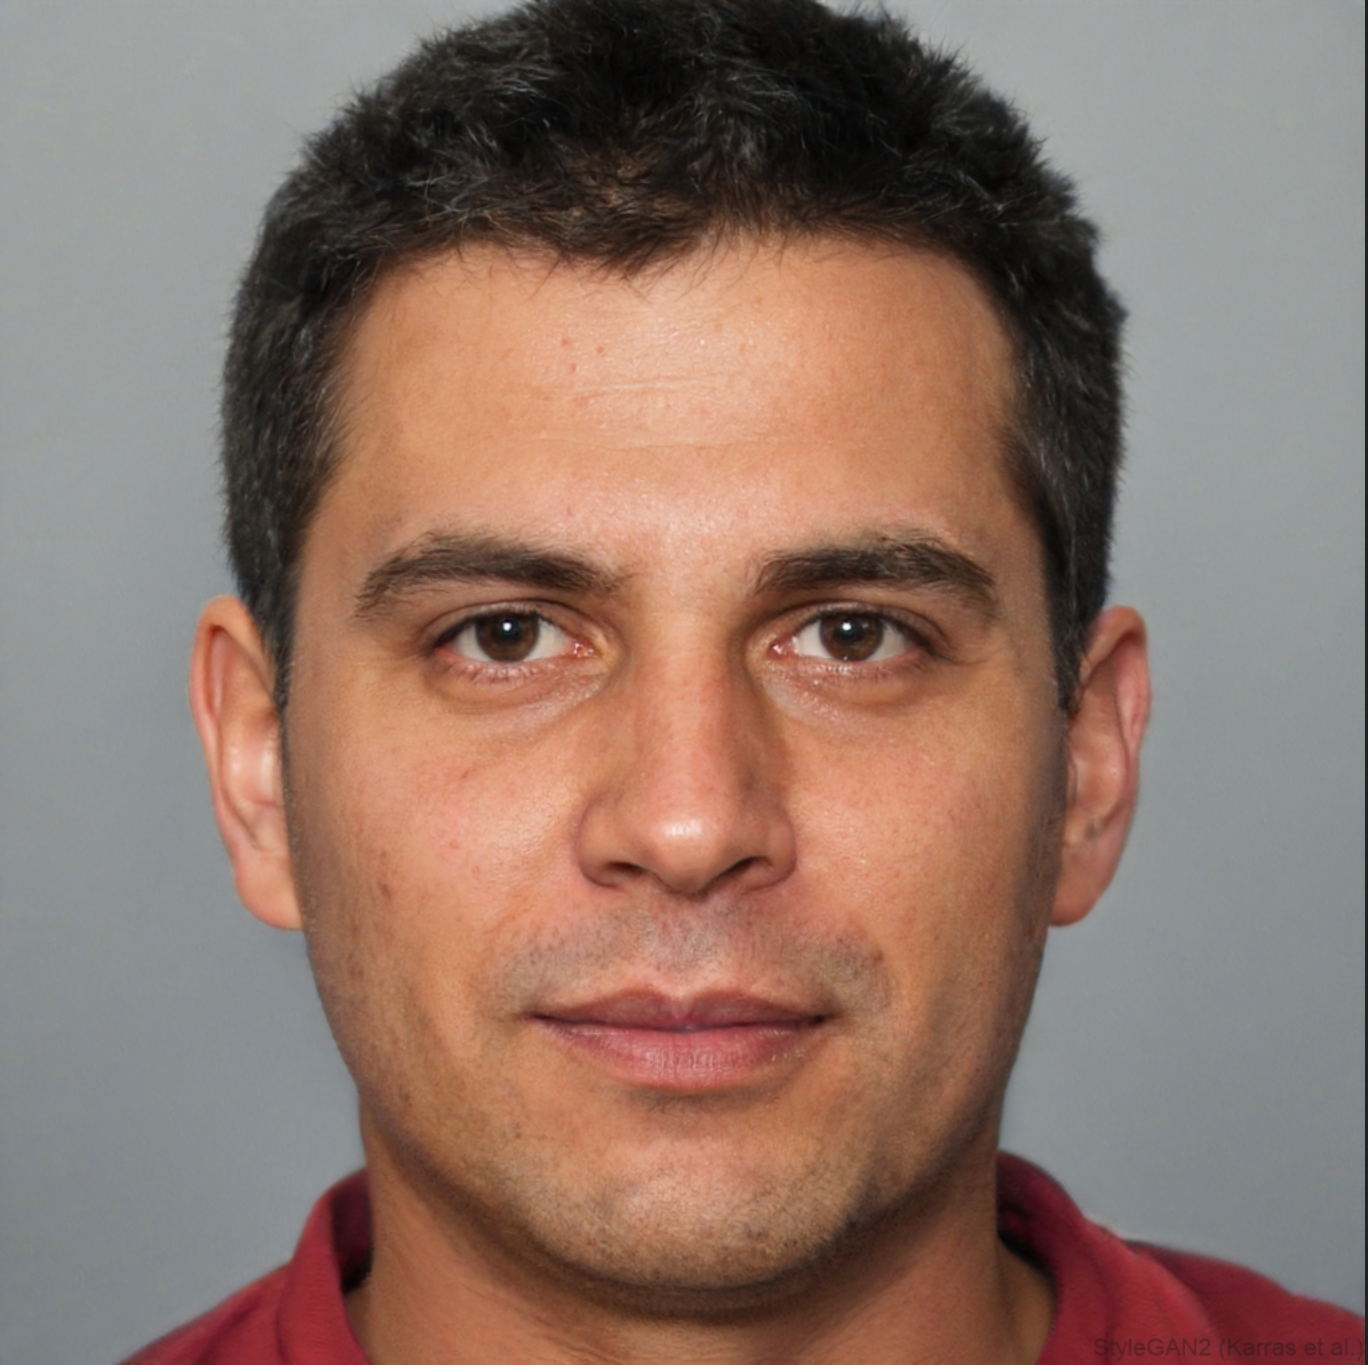
\includegraphics[width=0.5\linewidth]{img/this_person_doesntexist.png}\\
                \caption{ist diese Person real?}
            \end{figure}

        \column{0.4\textwidth}
            \begin{figure}
                \centering
                
\includegraphics[width=0.5\linewidth]{img/qr_personnotexist.png}\\
                \caption{Gerne ausprobieren :)}
            \end{figure}
    \end{columns}
        \
\end{frame}

\begin{frame}
    \frametitle{GAN - generative adversarial network}
         \begin{figure}
                \centering
                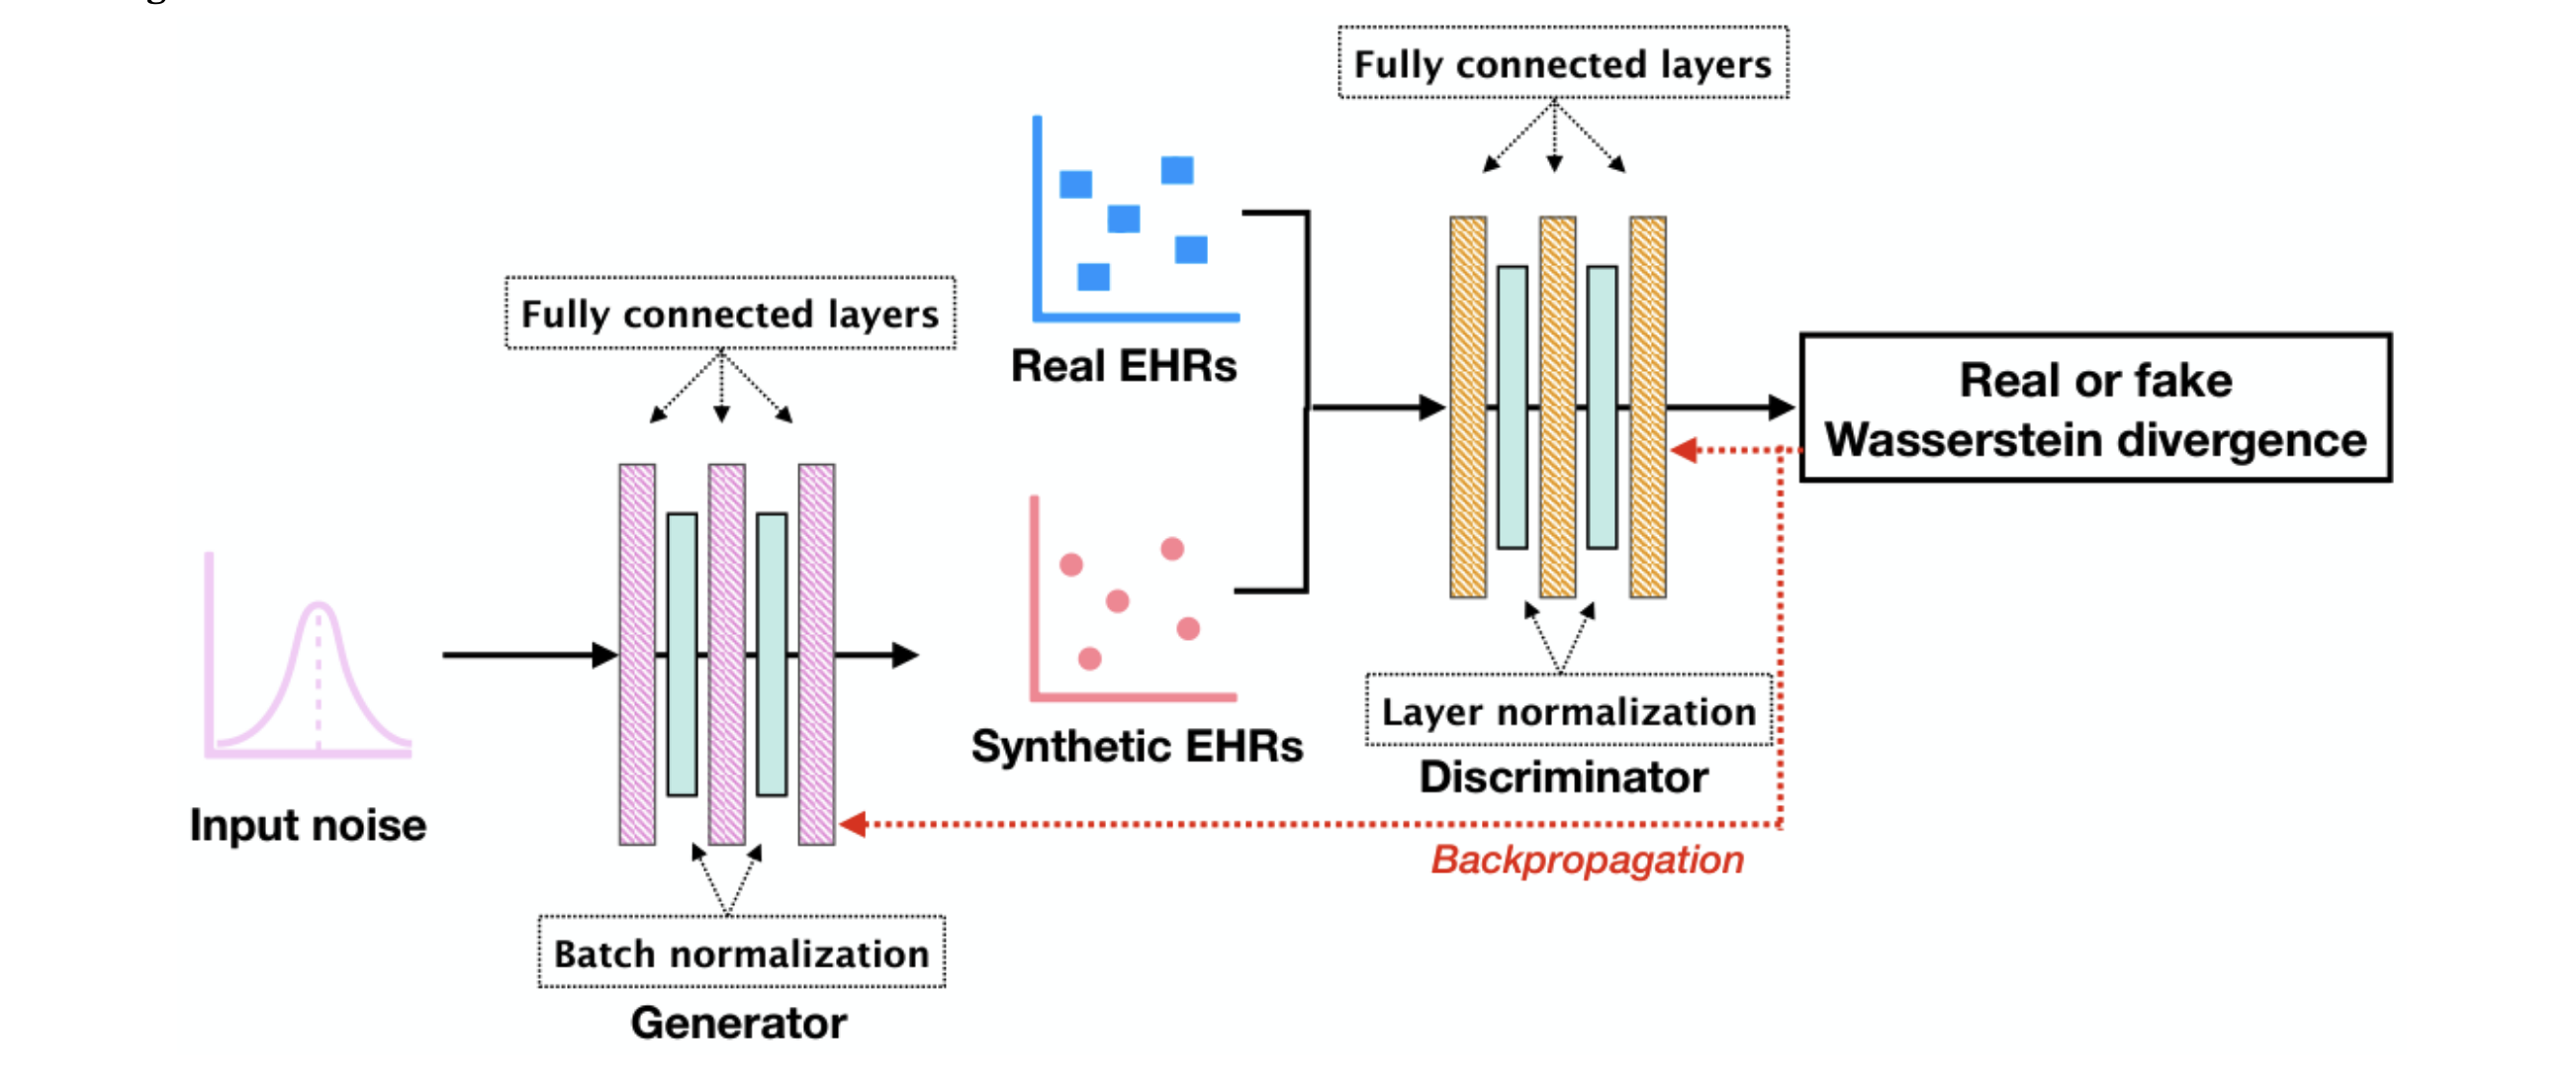
\includegraphics[width=0.7\linewidth]{img/gan_architecture.png}\\
                \caption{Aufbau GAN \parencite{yan_generating_2024}}
            \end{figure}
        \begin{columns}[T] % T = top aligned
        \column{0.48\textwidth}
           \begin{center}
                \tiny
                \begin{tabular}{lccccc}
                    \toprule
                    Pixel (1 Farbkanal) & x0 & x1 & x2 & ..  \\
                    \midrule
                    y0 & 0 & 244 & 123 & ...  \\
                    y1 & 10 & 246 & 100 & ...  \\
                    ...  & 119 & 7.4 & 78 & ... \\
                    \bottomrule
                \end{tabular}
            \end{center}

        \column{0.48\textwidth}
            \begin{center}
                \tiny
                \begin{tabular}{lccccc}
                    \toprule
                    Alter & Geschlecht & Blutdruck & Gewicht & Raucher  \\
                    \midrule
                    12 & F & 7.5 & 80 & Nein  \\
                    48 & M & 7500 & 0.08 & Ja  \\
                    27 & D & 7.4 & 78 & Nein \\
                    \bottomrule
                \end{tabular}
            \end{center}
    \end{columns}
\end{frame}

\begin{frame}
    \frametitle{CTGAN - conditional tabular GAN}
        \begin{figure}
                \centering
                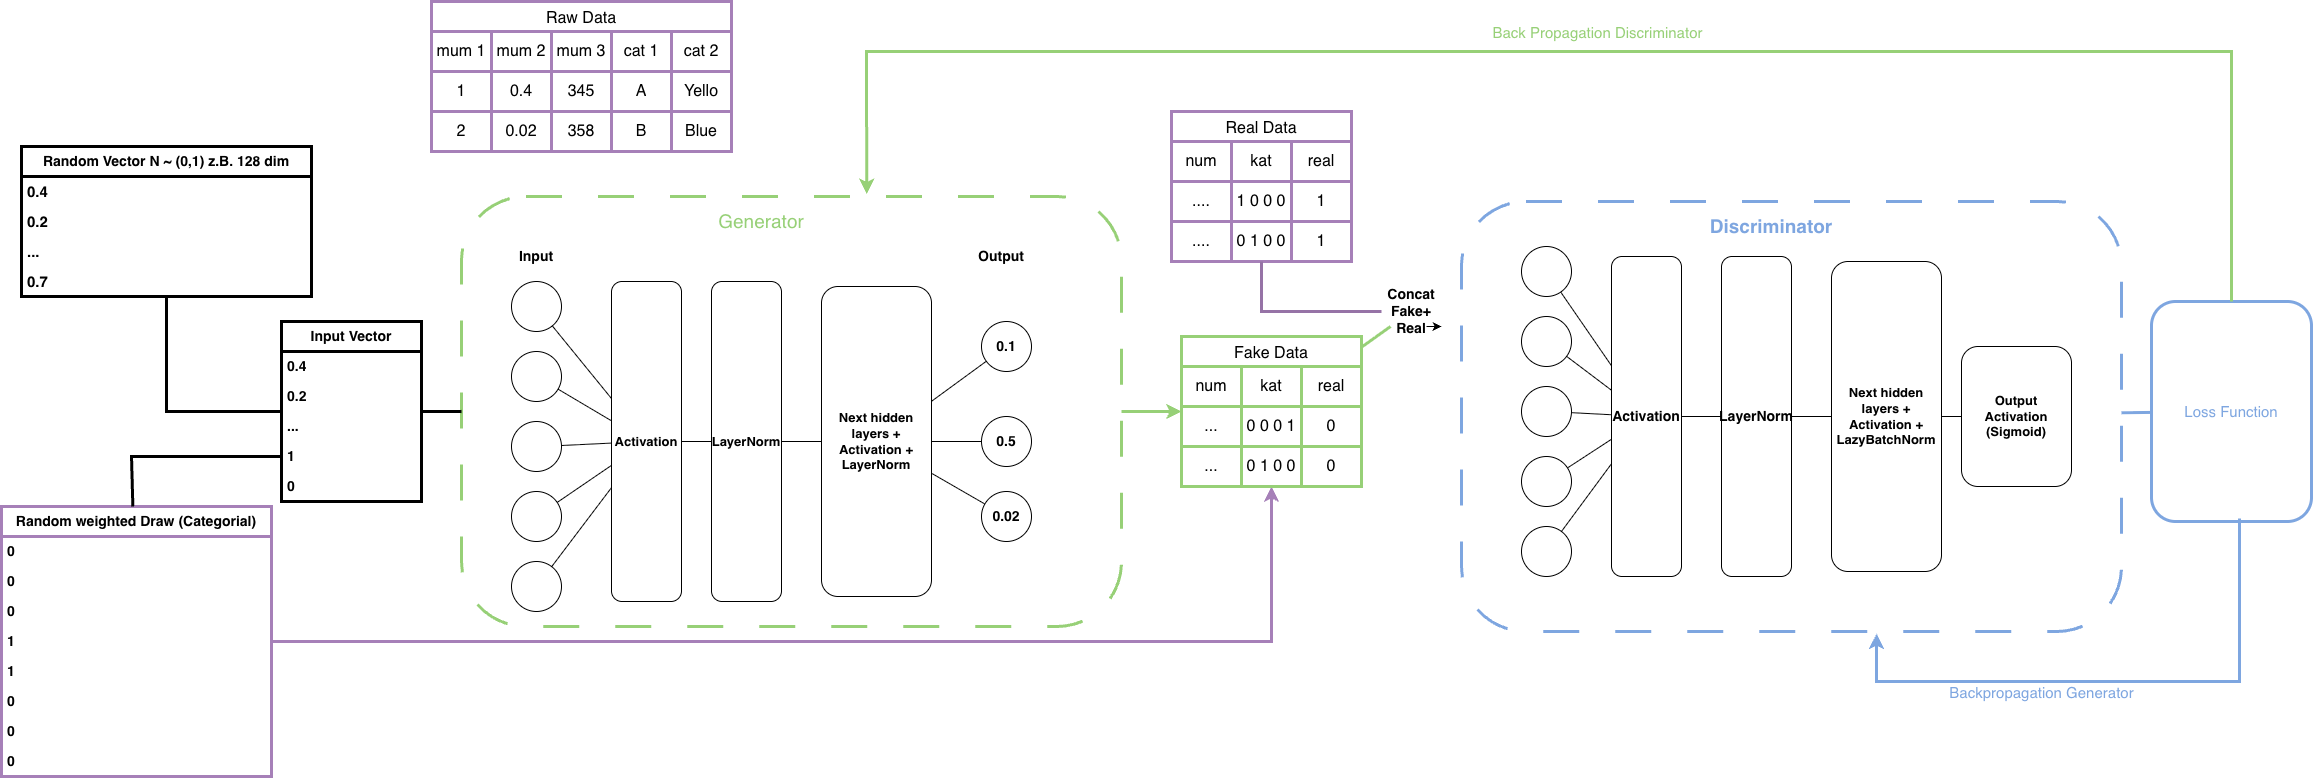
\includegraphics[width=0.95\linewidth]{img/ctgan_layout.drawio.png}\\
                \caption{Aufbau CTGAN}
            \end{figure}
\end{frame}

\begin{frame}
    \frametitle{Come with me if you want to live}
        \begin{center}
                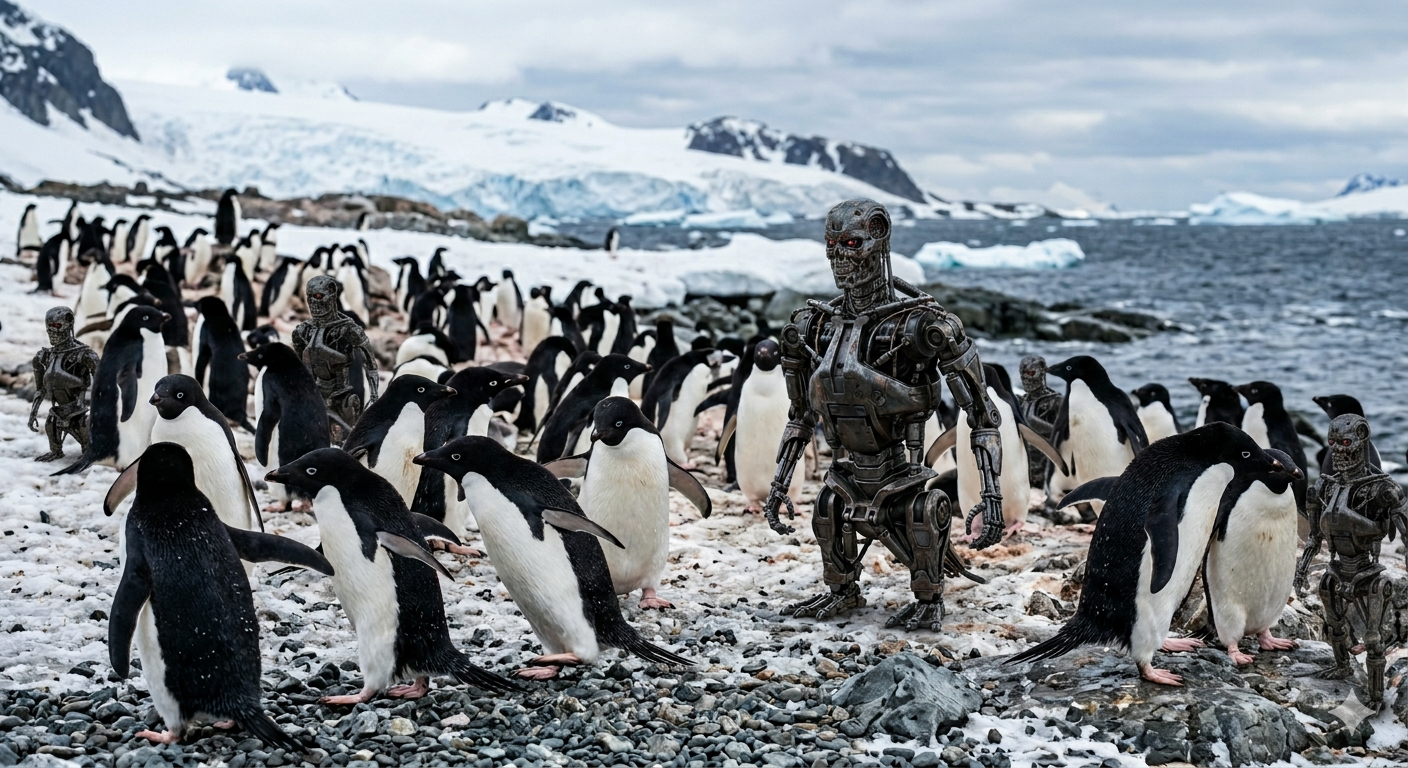
\includegraphics[width=0.8\linewidth]{img/synthetic_penguins.png}\\
                {\scriptsize Abb. 2 Generating Synthetic Electronic Health Record Data Using Generative Adversarial Networks: Tutorial}
            \end{center}
\end{frame}

\begin{frame}
    \frametitle{Training}
        \begin{columns}[T] % T = top aligned
        \column{0.48\textwidth}
           \begin{center}
                \tiny
                \begin{itemize}
                    \item Preprocessng
                    \item Training
                \end{itemize}
            \end{center}

        \column{0.48\textwidth}
            \begin{center}
                 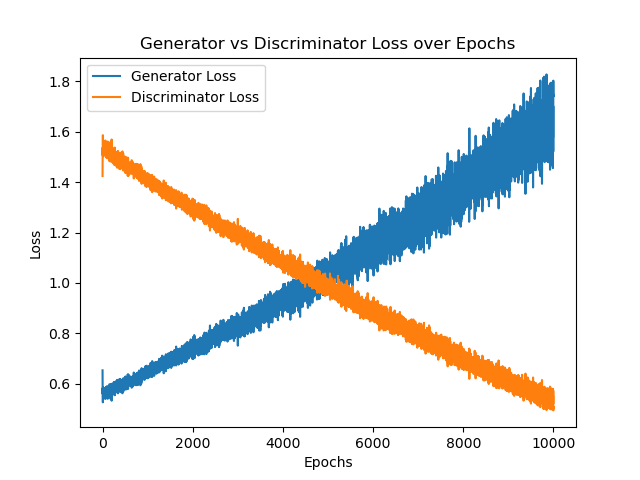
\includegraphics[width=0.7\linewidth]{img/Gen_lossvsdisc_loss.png}\\
                {\scriptsize Abb. 2 Generator vs Discriminator Loss}
            \end{center}
    \end{columns}
\end{frame}

\begin{frame}
    \frametitle{Ergebnisse}
       \begin{columns}[b]
        \column{0.48\textwidth}
            \begin{figure}
                \centering
                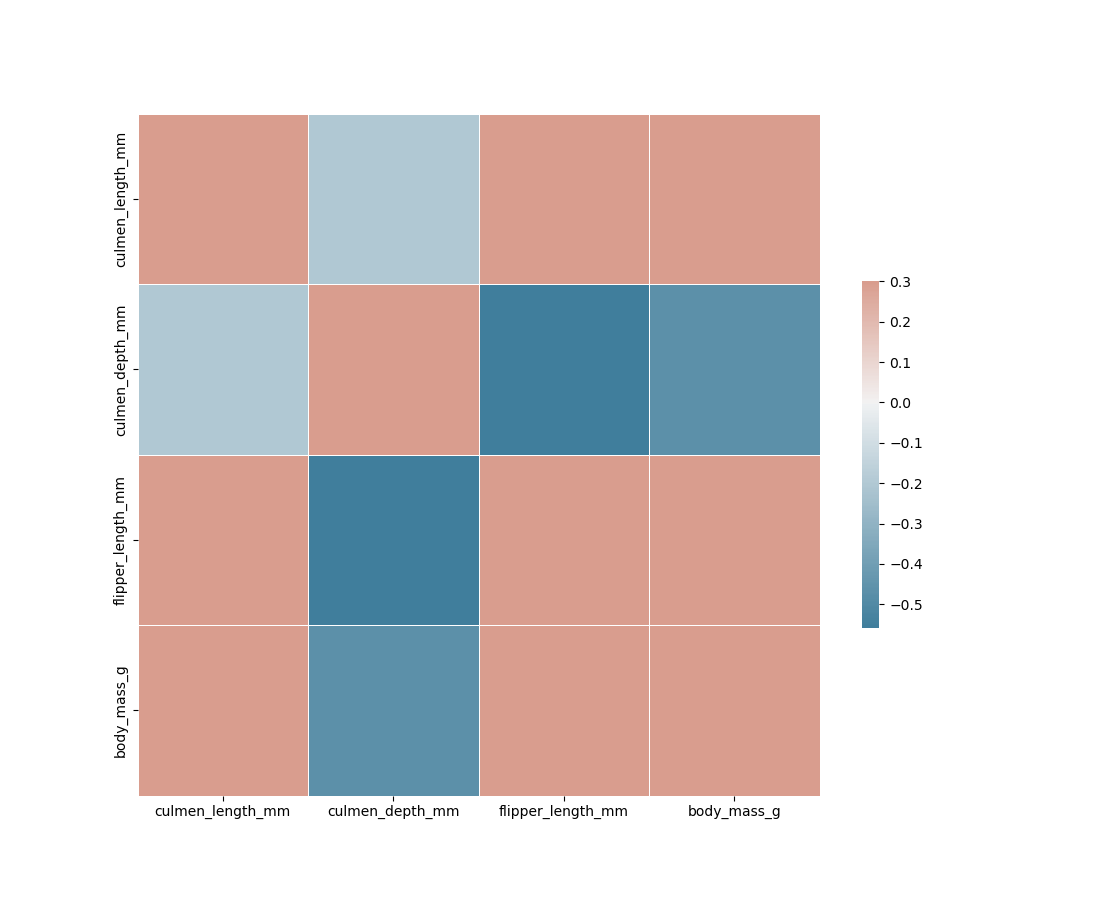
\includegraphics[width=0.5\linewidth]{img/corr_map_real.png}
                \caption{Korrelation Real}
            \end{figure}
            
        \column{0.48\textwidth}
            \begin{figure}
                \centering
                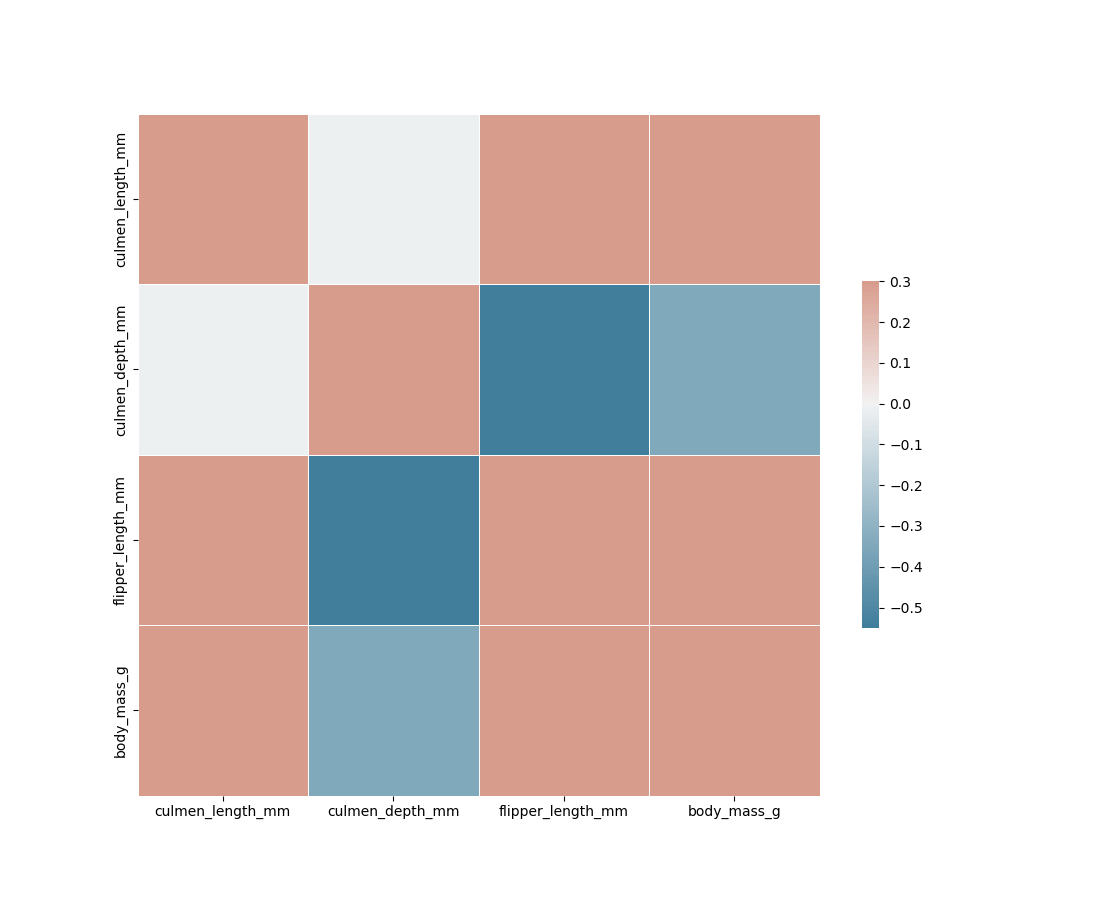
\includegraphics[width=0.5\linewidth]{img/corr_map_fake.png}
                \caption{Korrelation Fake}
            \end{figure}
    \end{columns}

    \vspace{0.2cm}

    \begin{columns}[b]
        \column{0.48\textwidth}
            \begin{figure}
                \centering
                
\includegraphics[width=0.5\linewidth]{img/screeplot.png}
                \caption{Screeplot}
            \end{figure}
            
        \column{0.48\textwidth}
            \begin{figure}
                \centering
                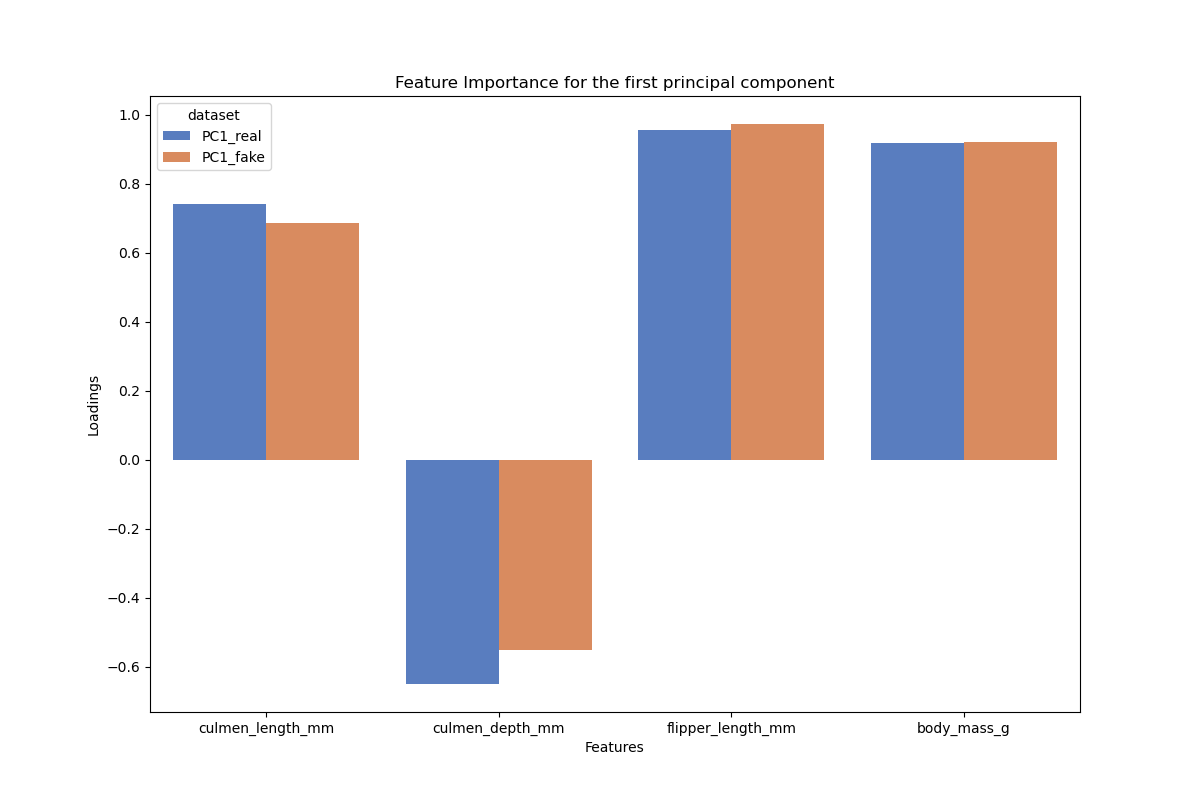
\includegraphics[width=0.65\linewidth]{img/loadings.png}
                \caption{Loadings}
            \end{figure}
    \end{columns}
\end{frame}

\begin{frame}
    \frametitle{Ergebnisse}
    \begin{columns}[b] % T = top aligned
        \column{0.49\textwidth}
           \begin{figure}
            \centering
            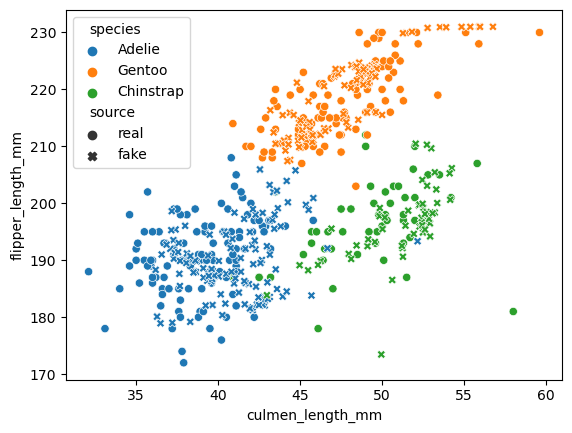
\includegraphics[width=0.7\linewidth]{img/fake_penguin_data.png}
            \caption{Generator vs Discriminator Loss}
        \end{figure}

        \column{0.48\textwidth}
            \begin{figure}
            \centering
            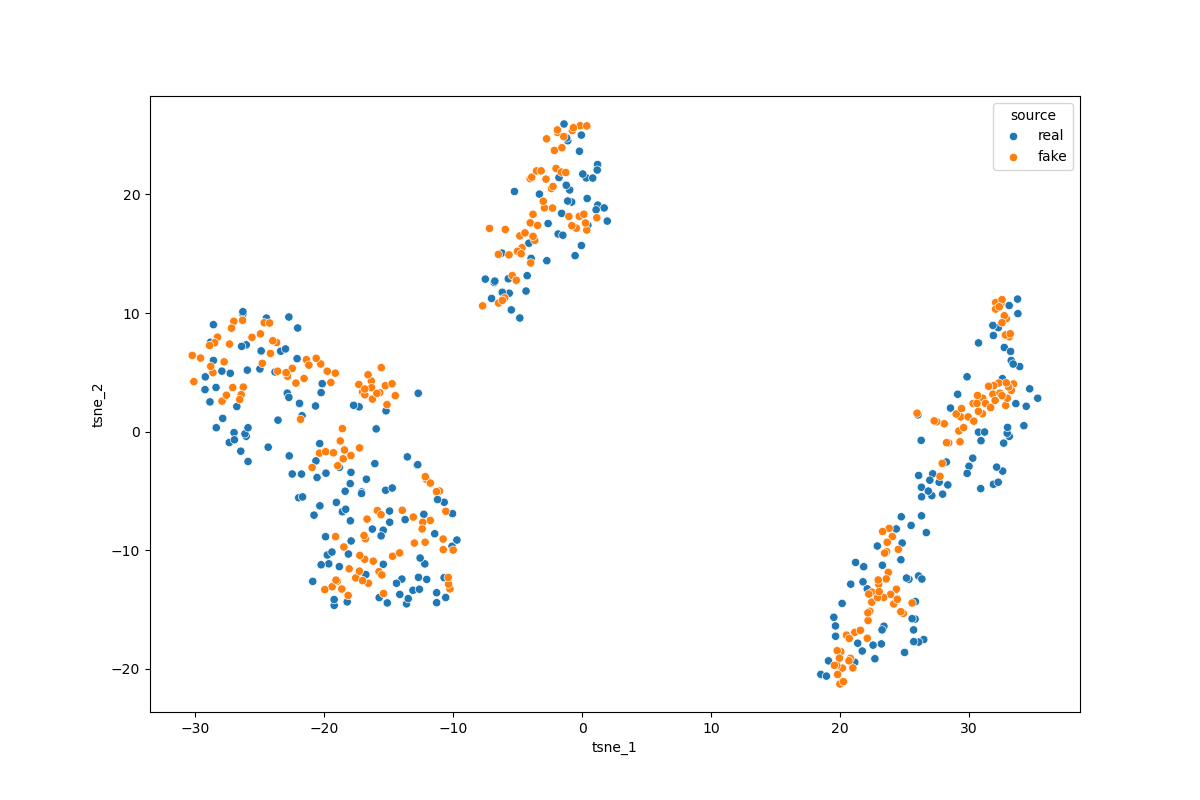
\includegraphics[width=0.9\linewidth]{img/tSNE.png}
            \caption{t-SNE Visualisierung}
        \end{figure}
    \end{columns}
\end{frame}



\begin{frame}
    \frametitle{}
        \
\end{frame}

\section{Table Diffusion}

%----------------------------------------------------------------------------------------
%\section{Probleme \& Herausforderungen}
%----------------------------------------------------------------------------------------


\begin{frame}
    \frametitle{Funktionsprinzip Table Diffusion}

    \begin{columns}[T, totalwidth=\textwidth]
        %----------------------------------
        \column{0.46\textwidth}\tiny
        \textbf{Tabelle: Messwerte unterschiedlicher Quellen}
        \vspace{0.3em}
        \begin{tabular}{lccccc}
            \toprule
            Quelle & M1 & M2 & M3 & M4 & Target \\
            \midrule
            Krankenhaus A & 120 & 7.5 & 80 & 1.2 & 100 \\
            Krankenhaus B & 12 & 7500 & 0.08 & 1200 & 100 \\
            Labor C & 119 & 7.4 & 78 & 1.1 & 100 \\
            \bottomrule
        \end{tabular}
        
        \vspace{1em}
        \textbf{HL7v2 vs FHIR}
          \begin{center}
           % \includegraphics[width=0.7\linewidth]{img/fhir_network.png}\\
           % {\scriptsize Abb. 2 FHIR Network }
        \end{center}
        %\vspace{0.1em}
       

        %----------------------------------
        \column{0.46\textwidth}\tiny
        \textbf{FHIR als Netzwerk}
        \vspace{0.3em}
        \begin{center}
           % \includegraphics[width=0.75\linewidth]{img/hl7v2.png}\\[0.5em]
           % \includegraphics[width=0.75\linewidth]{img/fhir.png} \\
           % {\scriptsize Abb. 3 HL7v2 vs FHIR}
        \end{center}
    \end{columns}
\end{frame}

\begin{frame}
    \frametitle{Wie funktioniert ein CTGAN}
        \
\end{frame}

\begin{frame}
    \frametitle{Wie funktioniert ein CTGAN}
        \
\end{frame}

%----------------------------------------------------------------------------------------
\section{Ausblick und Diskussion}
%----------------------------------------------------------------------------------------

\begin{frame}
    \frametitle{Andere Möglichkeiten zur synth. Datenerzeugung}
    \begin{itemize}
        \item SimbaML - simulation based machine Learning
        \item TVAE
        \item LLM
        \item "Ohne Standards bleiben Daten Inseln – mit Standards werden sie ein Netzwerk.
    \end{itemize}
\end{frame}

\begin{frame}
    \frametitle{Zusammenfassung}
    \begin{itemize}
        \item Synthetische Daten Mimiken reale Daten
        \item Es gibt keine einheitlich akzeptierte Metrik (Bewertungskriterien)
        \item Use Case sollte klar definiert werden
        \item Viele Wege (Methodiken) führen nach Rom (zum Ergebnis)
        \item CTGAN: funktioniert wie zwei Gegenspieler, wobei Generator aus Rauschen Fake Daten erzeugt und versucht Diskriminator auszutricksen
        \item Table Diffusion: neuronales Netz lernt wie Daten verrauscht werden 
    \end{itemize}
\end{frame}


%----------------------------------------------------------------------------------------
\section{Quellen}
%----------------------------------------------------------------------------------------

\begin{frame}
    \frametitle{Quellen}   
    \renewcommand{\bibfont}{\footnotesize} % Literaturverzeichnis etwas kleiner machen
    \printbibliography
\end{frame}

%----------------------------------------------------------------------------------------
%	SLIDE DE ENCERRAMENTO
%----------------------------------------------------------------------------------------

\begin{frame}
    \begin{center}
        {\Huge Vielen Dank für Eure Aufmerksamkeit!}
    \end{center}
\end{frame}

%----------------------------------------------------------------------------------------

\end{document}
